\documentclass{article}

\usepackage{graphicx}
\usepackage{subfig}
\usepackage{amsmath}
%\usepackage{amsmath,rotating}

\title{Three-dimensional Taylor Green}

\date{}

\begin{document}

\maketitle

\section{Introduction}
The Taylor-Green vortex at a Reynolds number of 1600 is a configuration 
commonly studied flow that captures elements of rudimental turbulence generation and 
decay~\cite{taylorGreen}, and serves as a case for a high-order workshop~\cite{hillewaert2012}. 
Unstructured, low-Mach numerical approaches were presented in~\cite{domino2019} using a series of 
homogenous topologies consisting of the following: Hex8, Hex27, Tet4, Pyramid5, and Wedge6.

The complete flow regime is marked by three phases that are described: Phase 1: viscous effects 
with small-scale laminar and organized structures are found; Phase 2: viscous (diffusion) effects 
dominating with accompanying stretching of vortex lines, and Phase 3: a break-up and is nearly 
isotropic in nature. Generally, for this simulation student, an explicit LES sub-grid stress model 
is omitted.  

The initial condition for the three-dimensional flow field is as follows:
%
\begin{eqnarray}
u_x &=& u_o sin(\frac{x}{L})cos(\frac{y}{L})cos(\frac{z}{L}), \nonumber \\
u_y &=& -u_o cos(\frac{x}{L})sin(\frac{y}{L})cos(\frac{z}{L}), \nonumber \\
u_z &=& 0, \nonumber \\
p &=& p_o + \frac{\rho_o u_o^2}{16}\left(cos(\frac{2x}{L}) + cos(\frac{2y}{L})\right)\left(cos(\frac{2z}{L})+2\right).
\end{eqnarray}

The quantities of interest for this simulation study is the temporal evolution of the kinetic energy, $E_k$, that
is integrated over the full domain at each time step. The energy-based dissipation rate 
given by $\epsilon_1 = -\frac{dE_k}{dt}$. 
The integrated enstrophy, $\zeta$ is defined by (in a low-Mach flow), $\epsilon_2 = \frac{2 \mu}{\rho_o} \zeta$,
where,

\begin{equation}
\zeta = \frac{1}{\rho_o V} \int_\Omega \frac{1}{2}\rho \omega_k \omega_k d\Omega.
\end{equation}
%
For more details, see~\cite{bullAndJameson2015}.

\section{Domain}
The simulation is run in a periodic square box of $-\pi L \leq x,y,z \leq \pi L$ with $L$ equal to unity. The simulation
is allowed to evolve from this initial condition over 20 characteristic convection time scales (defined 
by $t_c = \frac{L}{u_o}$). For this configuration, peak dissipation occurs at approximately $8t_c$.

\subsection{Simulation Specification and Sample Results}
A sample Q-criterion set of images for a Taylor-Green Re 1600 image appearing in~\cite{domino2019} is shown in 
Figure~\ref{fig:q}, while the set of converged results in this same paper are shown in Figure~\ref{fig:ek}.

\begin{figure}[!htbp]
  \centering
  {
   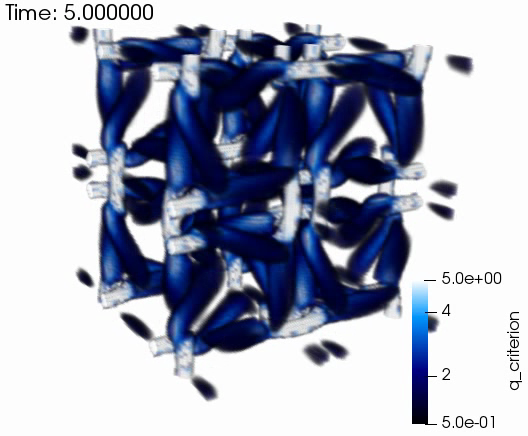
\includegraphics[height=1.5in]{images/tg_5s.png}
  }
  {
   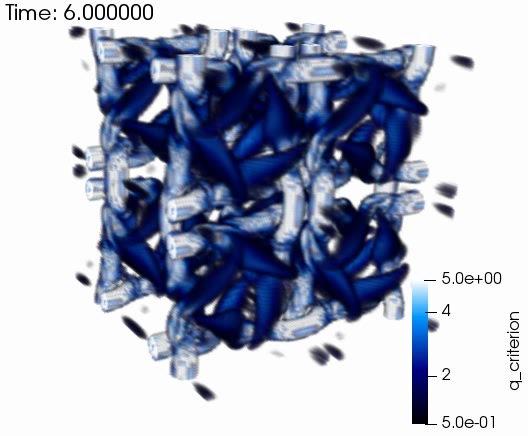
\includegraphics[height=1.5in]{images/tg_6s.png}
  } \\
  {
   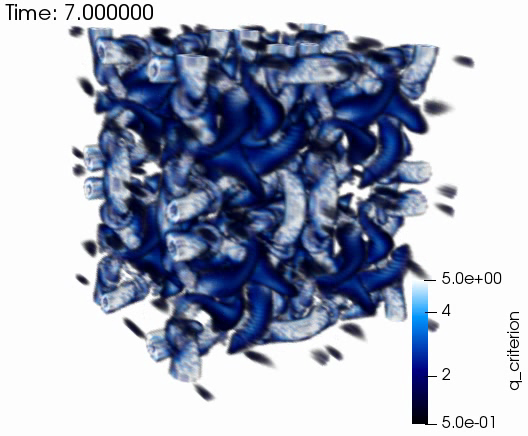
\includegraphics[height=1.5in]{images/tg_7s.png}
  }
  {
   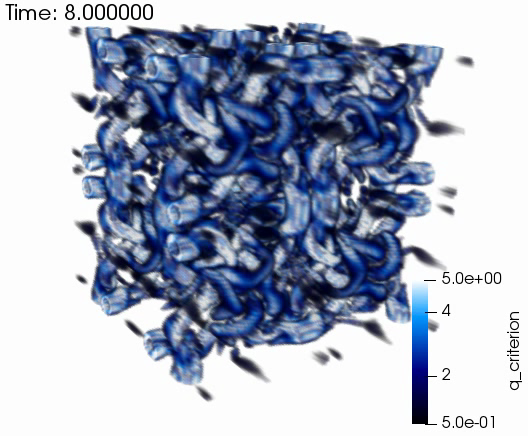
\includegraphics[height=1.5in]{images/tg_8s.png}
  }
  \caption{Three-dimensional Q-criterion volume rendered Taylor-Green representative time series at 5, 6, 7, and 8 seconds.}
  \label{fig:q}
\end{figure}

\begin{figure}[!htbp]
  \centering
  {
   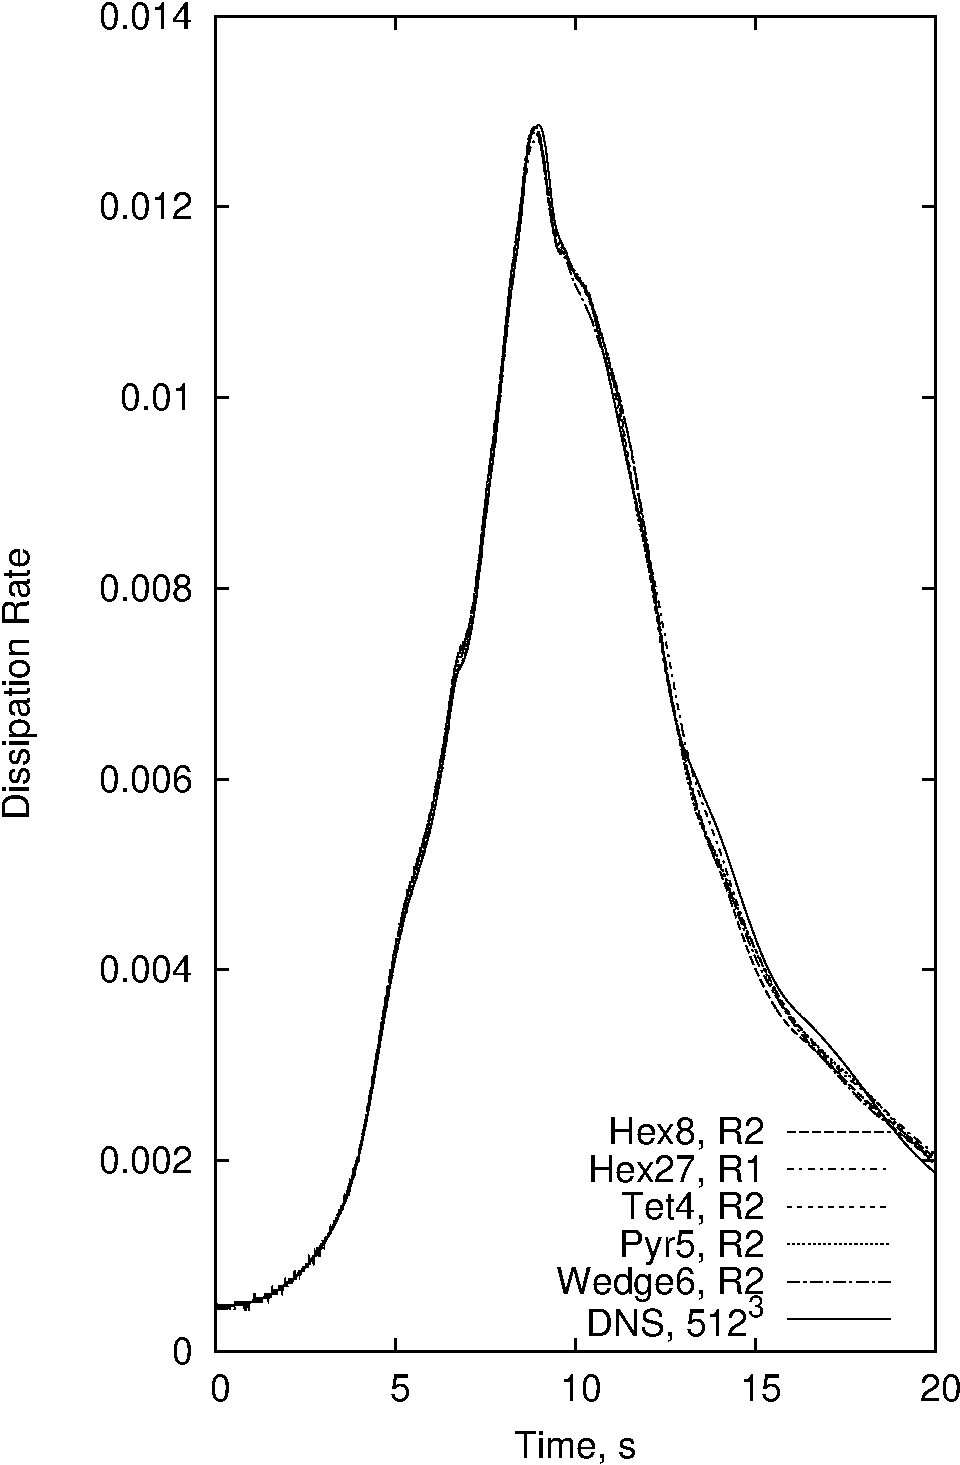
\includegraphics[height=4.0in]{images/tg_diss_hex8_tet4_pyr5_wedge6_R2_CU-crop.pdf}
  }
  \caption{Turbulence dissipation rate temporal plot for the series of mesh refinements in~\cite{domino2019}. In this
study, the baseline (R0) Hex8 mesh spacing of $\frac{2\pi}{100 L}$, i.e., $100^3$ elements was used.}
  \label{fig:ek}
\end{figure}

\subsection{Meshes}
The set of meshes provided in the mesh directory are as follows:

3d\_hex8\_taylor\_green\_0p2.g, 3d\_tet4\_taylor\_green\_0p2.g, and 3d\_tet4\_taylor\_green\_0p4.g. The 
mesh named ``0p4'' uses a 0.4 element length scale that can be useful for trouble shooting the monolithic 
implementation. Note that most peer-reviewed results appearing in the open literature exercise meshes 
that, even for a coarsest mesh spacing reported, are far more refined than the meshes provided in this study. 
However, the prime motivation for this exercise is to learn more about fully implicit solver approaches
in the low-Mach limit.

\section{Discussion Points}

There are several interesting activities associated with this sample case including
the points captured below. 

\begin{itemize}
	\item Document the appropriate equations for this conceptual model problem. Feel free to enforce the incompressible
          	constraint since this approach simplifies the momentum time and viscous term.
	\item Run the pressure projection input file (modified to run at least to 20 seconds), while post-processing the integrated 
		kinetic energy and dissipation plots. For the reference DNS of~\cite{hillewaert2012}, see the ``data''  directory.
        \item Implement an interior monolithic momentum and continuity kernel that captures the equation contributions indentified 
        		in the above first step. As a hint, this kernel should look 
          	very much like a combination of the segregated continuity (ContinuityAdvElemKernel) 
          	and momentum (MomentumAdvDiffElemKernel and MomentumMassElemKernel) classes, while noting that the total 
		size of the system is $nDim+1$.  In the LowMachMonolithicEquationSystem class, note that a single contribution is expected 
		by the name of: uvwp\_time\_advection\_diffusion (a consistent-mass kernel) or uvwp\_lumped\_time\_advection\_diffusion 
		(a lumped-mass kernel). Explore the usage of pressure stabilization in the momentum mass flow rate expression, in addition 
		to using the "old" values for the momentum and projected nodal pressure gradient field. You may also explore other forms of the
		advection form, although do not worry about implementing a limited upwind operator.
	\item Compare and contrast the simulation timings between the pressure projection and monolithic implementation. 
	\item $Optional$ As time permits, perform any mesh refinement and comment on the sensitivity of the QoIs.
	\item $Optional$ Perform any appropriate code verification using, for example, the convecting Taylor Vortex analytical solution
		on a periodic domain using your newly coded monolithic implementation.		
\end{itemize}


\bibliographystyle{unsrt}
\bibliography{3d_tet4_taylor_green_0p2}

\end{document}
